\section{Methods}
\begin{figure}
\centering
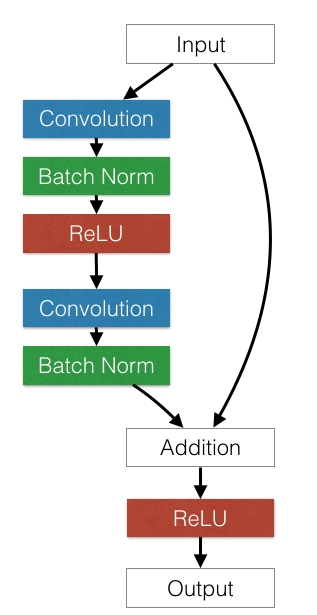
\includegraphics[width=0.4\columnwidth]{img/resnet}
\caption{
ResNet networks are characterized by skip connections, each of which bypasses several convolution layers \cite{gross2016training}.}
\label{fig:resnet}
\end{figure}

Our approach utilizes transfer learning, a well documented technique in the Deep Learning community as well as the broader field of Artificial Intelligence \cite{pan2010survey}.
Transfer learning involves repurposing models built for related, but distinct, problems. The original models serve as starting points for new models to be trained from.
This allows us to exploit knowledge gained from the original problem, without having to go through the process of learning it again in the new model. 
To incorporate transfer learning into our project, we utilize the ResNet \cite{he2016deep} architecture as a static feature extractor and train a single final fully connected layer to perform classification.
In some experiments, we perform fine tuning over all of the ResNet component's parameters in addition to the single final fully connected layer.
The ResNet architecture is designed for image classification and detection problems.
Deep feed-forward convolutional networks can suffer from a vanishing gradient problem where training stagnates due to error signal dissipation \cite{gross2016training}.
The ResNet architecture addresses this problem by including skip connections, each of which bypasses several convolutional layers \cite{he2016deep}.
At the end of a residual block, the output of the convolutional layers and the skip connection are summed \cite{gross2016training}.
By providing a direct shortcut for error signal to backpropagate through the network, these skip connections help to address the vanishing gradient problem.
Figure \ref{fig:resnet} provides a schematic depiction of a residual block.
ResNet architectures are composed of many such blocks.

\subsection{Preprocessing}

To meet the assumptions of the pretrained model components we used, we scaled images to 224 pixels by 224 pixels and performed the following channel normalizations, where $r$, $g$, and $b$, correspond to the red, green, and blue channels respectively:
\begin{align*}
r
&\sim
\mathcal{N}(0.485, 0.229) \\
g
&\sim 
\mathcal{N}(0.456, 0.224) \\
b
&\sim
\mathcal{N}(0.406, 0.225).
\end{align*}

To keep our work computationally tractable we work with just a subset of the entire Cdiscount dataset.
We restrict our work to two high-level categories and 20 of each high-level category's low-level categories.
We arbitrarily chose furniture and electronics as our high-level categories and then chose low-level categories to include based on the availability of adequate training data.
This reduced dataset comprises approximately 20,000 images, which were distributed roughly evenly between low-level categories.
Each low-level category had between 300 and 500 training examples.


\subsection{Approaches}
\begin{figure}
    \centering
    \begin{subfigure}[t]{0.55\columnwidth}
        \centering
        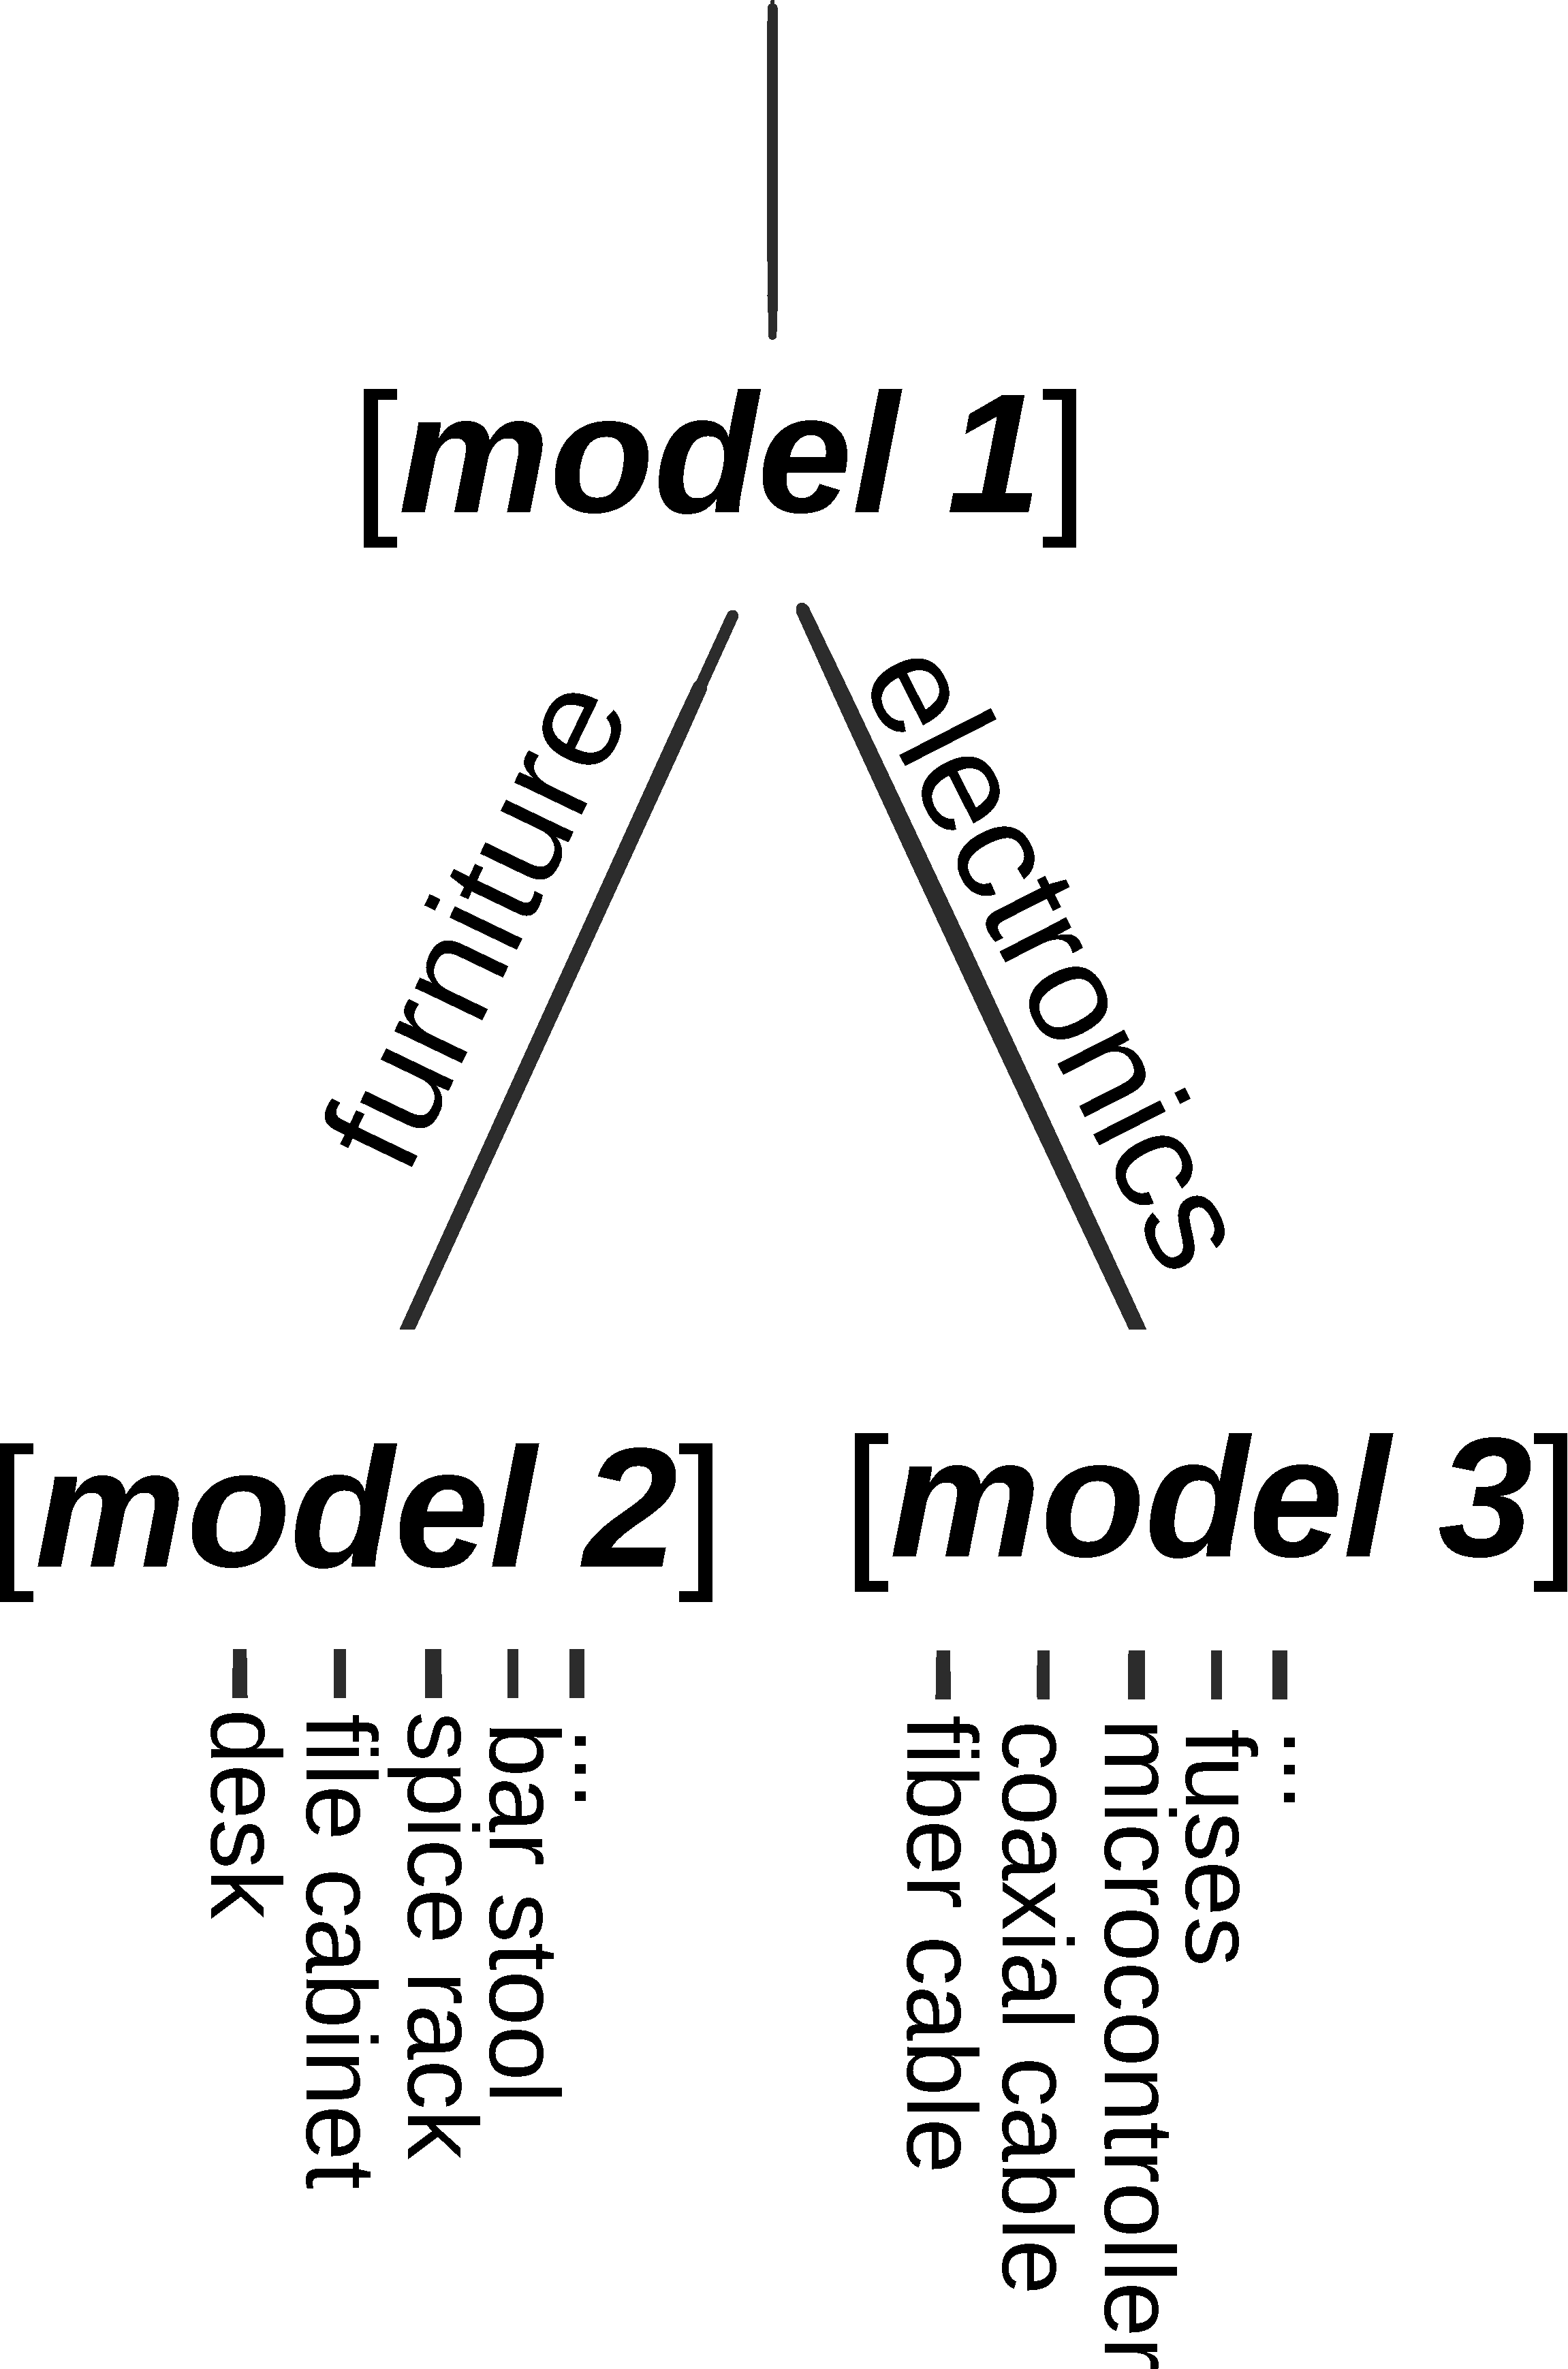
\includegraphics[width=\textwidth]{img/nested}
        \caption{nested models}
    \end{subfigure}%
    ~~~~~
    \begin{subfigure}[t]{0.40\columnwidth}
        \centering
        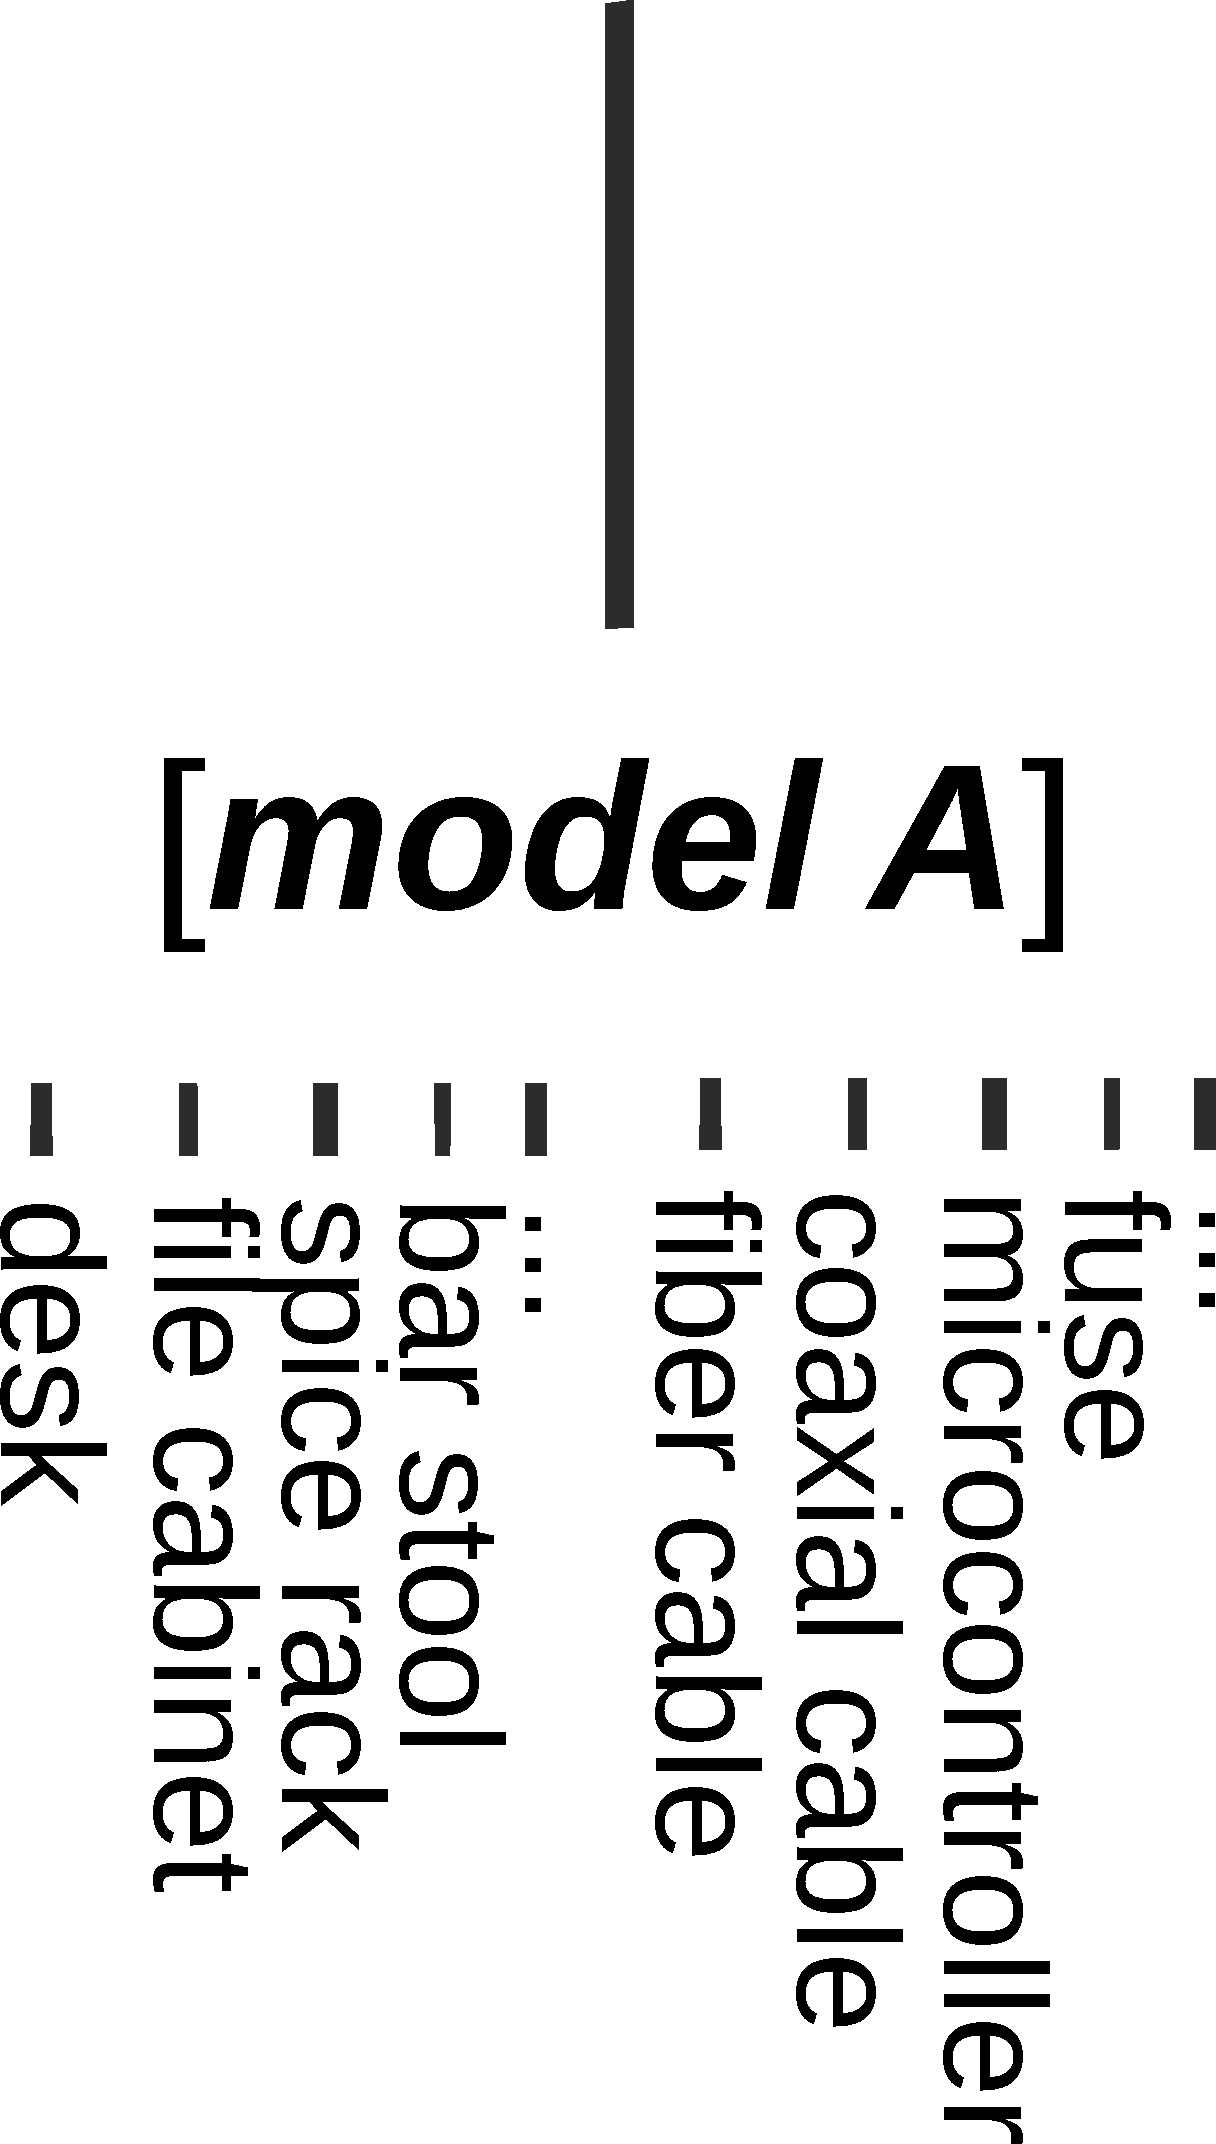
\includegraphics[width=\textwidth]{img/flat}
        \caption{flat model}
    \end{subfigure}
	\caption{
Schematic diagrams of the two approaches compared in this paper.
}
	\label{fig:approaches}
\end{figure}

We set out to compare the performance of two approaches to hierarchical image classification.
The first approach uses an ensemble of three models --- 1, 2, and 3 --- to perform classification.
Model 1 performs a classification between high-level categories.
With our reduced dataset, this is a binary classification.
We call this model the binary classification model.
Model 2 performs a classification between low-level categories for images classified by model 1 as belonging to a particular high-level category, in our case furniture.
We call this model the furniture-only model.
Model 3 performs a classification between low-level categories for images classified by model 1 as belonging to the other high-level category, in our case electronics.
We call this model the electronics-only model.
With our reduced dataset, models 2 and 3 both perform 20-class classification.
We refer to this approach the hierarchical models approach.

The second approach uses a single model to directly classify images between all low-level categories.
With our reduced dataset, this model performs 40-class classification.
Given the strictly hierarchical nature of cDiscount's classification scheme, the higher-level classifications of the image can be directly inferred from the low-level classification performed under this second approach. 
We call this approach the flat model approach.
Figure \ref{fig:approaches} provides a side-by-side schematic comparison of the hierarchical models and the flat model approaches.

\subsection{Implementation}

We use PyTorch and Torchvision to implement our experiments \cite{paszke2017pytorch}.
We used the ResNet18 model available through Torchvision, which has 11,689,512 trainable parameters when we perform fine tuning.
The final classification layer has 20,480 parameters for the flat model, 1,024 parameters for the binary classification model, and 10,240 parameters for the furniture-only and electronics-only models.  
The flat approach employs just one ResNet18 model.
However, the hierarchical approach employs three ResNet18 models and therefore entails three times the number of trainable parameters. 
We trained our models on a Google Cloud Compute virtual machine with a Nvidia Tesla K80 GPU.
Training our models consumed a total of 24 hours of compute time with this setup.

The scripts we used to analyze and visualize the Cdiscount dataset are hosted at \url{https://github.com/mmore500/cdiscount-datavis}.
Our code for dataset preparation, model design, model training, and comparison of classification accuracy between the flat model and the hierarchical models approaches is hosted at \url{https://github.com/ianwhale/cse891}.
